\documentclass[a4paper,twocolumn,twoside,10pt]{ranlp}
\usepackage{epsfig}
\usepackage{latexsym}
\usepackage[usenames]{color}
\usepackage{times} 
\usepackage{verbatim}
\usepackage{multirow}

\begin{document}
\title{Event Detection in Blogs using Temporal Random Indexing}


\author{ {\bf David Jurgens} and {\bf Keith Stevens} \\
University of California, Los Angeles \\
4732 Boelter Hall \\
Los Angeles, CA 90095 \\
\email{\{jurgens,\ kstevens\}}{cs.ucla.edu} \\
}

\date{}

\maketitle

\thispagestyle{empty}        \pagestyle{empty}

\begin{abstract} 

Automatic event detection aims to identify novel, interesting topics as they are
published online.  While existing algorithms for event detection have focused on
newswire releases, we examine how event detection can work on less structured
corpora of blogs.
%
The proliferation of blogs and other forms of self-published media have given
rise to an ever-growing corpus of news, commentary and opinion texts.
%
Blogs offer a major advantage for event detection as their content may be
rapidly updated.  However, blogs texts also pose a significant challenge in that
the described events may be less easy to detect given the variety of topics, writing
styles and possible author biases.
%
We propose a new way of detecting events in this media by looking for changes in
word semantics.
%
We first outline a new algorithm that makes use of a temporally-annotated
semantic space for tracking how words change semantics.
%
Then we demonstrate how identified changes could be used to detect new events
and their associated blog entries.

\end{abstract}

\section {Introduction}

Automated event detection is a form of information retrieval where given a
time-ordered set of documents, an algorithm must select those which represent
recent news or changes to existing information.  An automated approach to event
detection has many practical applications; given the large amount of text being
written daily, readers want to be informed of which developments and topics are
the most recent and important without having to manually sift through all the
documents written on the topic.  In addition, a robust system should be able to
detect multiple kinds of events, such as international conflicts, product
releases or sports results.  The main challenge in automating this task is
detecting what makes a new document sufficiently novel to be described as a new
event.

Current event detection approaches have focused on identifying concrete events
that occur within newswire text\cite{kumaran04entityevent}.  However, in recent
years, blogs have become an important source of both news and commentary.  Unlike
news reports, blog content expresses a wide range of topics, opinions,
vocabulary and writing styles; the change in editorial requirements allows blog
authors to comment freely on local, national and international issues, while
still expressing their personal sentiment.  Accordingly, blogs offer a rich
opportunity for detecting events that may not be covered in traditional newswire
text.  These forms of self published media might also allow event detection
systems to identify developing events before official news reports can be written.

Several forms of event detection have focused on analyzing named entities, such
as ``Bill Clinton'' or ``Iraq,'' and the contexts or documents in which they
appear, e.g.
\cite{kontostathis04use,kumaran04entityevent,fortuna09visualization}.  We
propose a more general approach that looks at all words and their contexts,
rather than a predetermined set of words.  Specifically, we argue that event
detection can be done by measuring the semantic change in a word or phrase.  To
track changes in the semantics, we use a semantic space model of meaning, which
is an automated method of building distributed representations of word meaning.

Semantic space models of meaning offer three notable advantages for event
detection.
%
First, the models are capable of automatically determining the semantics of a
word by examining the contexts in which the word appears.  Such automated
understanding of semantics is required for analyzing these new sources of data
due to the much wider vocabulary used by authors.
%
Second, the models offer a well defined method for comparing the semantics
between words.  These semantic comparisons have been shown to be similar to
human judgments\cite{landauer97solution}.  We argue that reporting words which
have a notable changes in semantics should correlate well with a reader's
expectations of interesting developments.
%
Third, the models are well-established at detecting association such as synonymy
among words, which can allow models to detect events that are referred to by
multiple names.
%
Given these advantages, we introduce a new semantic space algorithm for
assessing how the meaning of a word changes through time for the purpose of
event detection.

We illustrate our approach to topic detection with a hypothetical example of the
product release of a toy named ``blick.''  At the start of the toy's popularity,
the word ``blick'' has not occurred before and therefore its semantics would be
undefined.
%
As ``blick'' appears in more blogs, the word acquires consistent semantics, and
the algorithm can report a new event for ``blick.''  Our approach differs from
simple occurrence monitoring in that we require the word to have a consistent
meaning; unless the algorithm is capable of determining what concepts the word
refers to, knowing that the word relates to an event is impossible.

However, consider detecting a second event for ``blick'' soon after its release
in which the toy is discovered to have toxic properties.  Since the toy's name
was already present in the blogs, the novelty of the name is not enough to
detect the point at which the toxic chemical was revealed.  However, our
approach, which looks at the semantic shift of words over time, would detect a
shift based on the new kinds of words that would be likely to co-occur with the
toy's name, e.g. toxicity, a toy recall, or lawsuit.  Intuitively speaking, this
approach associates news events with noticeable changes in both \emph{what}
authors talk about and \emph{how} they talk about those subject.

In this paper we present a new algorithm, Temporal Random Indexing, that
effectively captures the semantic changes for words and phrases over time.  We
first briefly review the semantic space model that underlies this approach and
then present the algorithm.  Following, we demonstrate several examples of
semantic change extracted from a large blog corpus and illustrate one method for
reporting the events.  

\section {Semantic Space Models}

Semantic space models of meaning are born from the distributed hypothesis: For
two words, their similarity in meaning is predicted by the similarity of their
distributions of co-occurring words\cite{harris68mathematical}, or as Firth puts
it, ``you shall know a word by the company it keeps,''\cite{firth57synopsis}.
Creating semantics from co-occurring words forms the basis for how our algorithm
represents changes in semantics.

\subsection{Semantics as Co-occurrence}

In a semantic space, a word's semantics are mapped to high dimensional vectors
in a geometric space.  The dimensions of the space represent distinctions
between the meanings of words; accordingly, words with similar semantics have
similar vector representations.  Semantic space representations have proven
effective at a variety of information retrieval tasks such as identifying
synonymous queries\cite{schutze97cooccurrence} and multi-language
retrieval\cite{littman98automatic,vinokourov2002finding}.  For a recent survey
of applications of semantic spaces to information retrieval see Cohen and
Widdows\cite{cohen09empirical}.  To illustrate the basics of co-occurrence based
semantic space models, we can further explore the example of ``blick'', the new
yet toxic toy.

Consider the documents describing ``blick'' when it is first introduced during a
holiday season.  A potential line from several blogs might read ``A perfect gift
this holiday season is blick, one of the newest toys available!''  Using a
simple co-occurrence semantic space, the semantics of ``blick'' would be a count
of how frequently it co-occurs with key words such as: gift, holiday, perfect
and toys.  Examining later blog posts written when this same toy is discovered
to have toxic elements, several posts might now have the line: ``the toxic
elements in blick make the toy dangerous.'' The semantics of the toy should now
focus primarily on the co-occurrence of words such as toxic and dangerous, and
should no longer be associated with positive words such as holiday and perfect.
Figure \ref{fig:ri-space} illustrates a simplified two-dimensional semantic
space and the changes to semantics that would occur as ``blick'' begins to
co-occur with toxic-related words.  A standard semantic space model would define
the semantics of the new toy as a combination of all co-occurrences, in this
case the positive new semantics and the negative semantics of toxicity.

\subsection{Random Indexing}

Using simple co-occurrence is rarely done in practice for large corpora.  In
such models, each unique word would be assigned its own dimension (corresponding
to co-occurrence with that word), which results in vectors with hundreds of
thousands to millions of dimensions.  Basing the number of dimensions on the
number of unique words is particularly problematic for blog corpora, as writers
frequently introduce misspellings, slang, or topic-specific jargon.
Accordingly, many approaches have focused on reducing the dimensionality of the
semantic space.  Dimensionality reduction often has the additional benefits such
as making the resulting vector more general, or reducing computation time.

Early successful approaches such as Latent Semantic
Analysis\cite{landauer97solution} use the Singular Value Decomposition (SVD) to
reduce the number of dimensions.  While the SVD results in significant
improvements in information retrieval, the fastest algorithms for the SVD are
O(mn$^2$) \cite{bau97numlinalg}, which make them impractical for large corpora.
Moreover, the SVD and other forms of principle component analysis must have the
entire corpus present at once, which makes it difficult to update the space as
new words and contexts are added.  This is particularly problematic for event
detection, as the corpus is expected to continuously grow as new events occur.

Random Indexing\cite{kanerva00random,sahlgren01vector} offers an alternative
method for reducing the dimensionality of the semantic space by using a random
projection of the full co-occurrence matrix onto a lower dimensional space.
Random Indexing operates as follows.  Each unique word is assigned an
\emph{index vector}, which is a random, sparse vector in a high dimensional
space, often 2000-10000 dimensions. The size of the index vectors sets the
number of dimensions used in the resulting semantic space.  Index vectors are
created such that any two arbitrary index vectors have a high probability of
being orthogonal.  This property is necessary to accurately approximate the
original word co-occurrence matrix in a lower dimension.  The semantics of each
word are calculated by summing the index vectors of all co-occurring words
within a small window of text.  Random Indexing works well in practice as the
dimensionality reduction occurs as the corpus is being processed, rather than
requiring an explicit step after all the corpus has been seen.

More formally, let $w$ be a focus word, $w_i$ be a co-occurring word with a word
distance of $i$ and $index(w_i)$ be the co-occurring word's index vector.  For
the current word, we define a window of size $n$ words before and after, which
are counted as co-occurring.  The semantics of $w$ are then defined as:
%
\begin{equation}
\label{eq:random_indexing}
semantics(w) = \sum_{\forall c \in D} \sum_{ -n \leq i \leq n} index(w_i)
\end{equation}
%
where $c$ is each occurrence of $w$ in the corpus $D$.


\begin{figure} 
  \center
  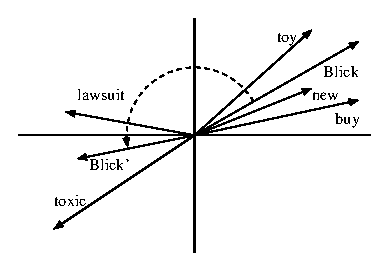
\includegraphics[width=.35\textwidth]{figures/example-semantic-space.eps} 
  \caption{Word semantics projected into two dimensions, illustrating the
    hypothetical change in meaning for ``blick'' based on its nearest neighbors}
  \label{fig:ri-space} 
\end{figure}

\subsection{Adding Time to Semantic Space Models}

Augmenting a semantic space with time has been recognized as an effective method
for tracking changes in semantics\cite{sahlgren08buzz}. Two methods have been
  used to add temporal semantics.  The first approach builds a separate semantic
  space for each specific time range.  Semantics are then compared across spaces
  by defining some common context which occurs in both spaces.  The second
  approach builds a single semantic space but provides the ability to segment it
  based on time.  The key difference between these approaches lies in the
  meaning of each semantic dimension; when multiple spaces are used, there is no
  guarantee that the specific semantic meaning associated with some dimension
  $i$ will be the same for dimension $i$ in another space.

Kontostathis et al.\cite{kontostathis04use} and Fortuna et
al.\cite{fortuna09visualization} have independently proposed two successful
semantic space algorithms that use the first approach of processing several
distinct corpora.  Both approaches collect several corpora which span unique
time ranges, and construct a semantic space for each corpus using LSA.  Using
LSA is a notable challenge as the space defined by LSA is based on the SVD of a
word $\times$ document matrix; with documents being unique to each time-span's
corpus, direct comparison of vectors between spaces is not feasible.

Kontostathis et al.\cite{kontostathis04use} use data mining to overcome the
change in dimension-meaning by first clustering the semantics from each year.
With this clustering, key attributes are extracted from several time ranges, and
significant differences are used to infer an event or trend.  In essence, vector
comparisons between the semantic spaces are bypassed by using cross-space
meta-statistics for each word generated from each space.  This approach is
limited to being an offline approach due to the costly machine learning
techniques, and is further limited by key sets of attributes.

Another approach for comparing semantics from semantic spaces has been
introduced by Fortuna et al.\cite{fortuna09visualization}.  Their approach
focused on finding key words that existed in multiple spaces, and defining a
concrete set of semantics for these landmark words.  As semantics from distinct
spaces are created, they can be evaluated according to their relation to these
landmark terms, and at any point in time, the words most closely associated to
the landmark provide terms describing events related to the landmarks.

Sagi et al. propose an alternate approach of uses a single corpus and includes
temporal semantics after generating an initial set of
semantics\cite{SagiSemanticDensity}.  This generates semantic vectors for a
corpus spanning many time ranges of interest and reducing dimensionality via
SVD.  Then, to develop temporal semantics for a term, documents from a specific
time range are used to generate temporal vectors through a process very similar
to Random Indexing; in this process the first set of semantic vectors generated
are used in place of index vectors when using equation
\eqref{eq:random_indexing}.

While these approaches allow for accurate representations of semantic shifts,
they face significant challenges when scaling to a large streaming set of
documents, due to a reliance on the SVD for dimensionality reduction.
Additionally, none of the algorithms are able to change the time-spans used for
analysis without reprocessing some portion of a corpus.  Given these
limitations, a computationally efficient modification to how a semantic space is
produced is necessary to permit more detailed analysis of changing semantics.

\section{Temporal Random Indexing}

Temporal Random Indexing (TRI) incorporates time by building a single semantic
space.  However, instead of using a word $\times$ semantics matrix, TRI uses a
word $\times$ semantics $\times$ time tensor.  Figure \ref{fig:tensor-space}
illustrates this change.  The time dimension records the semantic vectors of a
word for each time unit (e.g. a week or month).  

TRI offers three major advantages over existing models.  First, the semantic
space is built incrementally so new documents may be added at any time.  Second,
the tensor representation allows for arbitrary time-range comparisons.  Third,
we use a dimensionality reduction similar to that of Random Indexing, which
operates as the documents are processed, rather than all at once.  This results
in greatly reduced time and memory requirements compared to those methods that
rely on the SVD for dimensionality reduction.

To associate specific time values with semantics, TRI does not
immediately perform the summation as defined in equation
\eqref{eq:random_indexing}.  Instead TRI only accumulates the semantics for
contexts which occur in the same time period.  These time period semantics are
then stored in chronologically ascending order to produce a semantic slice for a
word.  The plane in figure \ref{fig:tensor-space} represents the semantic slice
of a single word, which covers all the time periods in which that word has been
observed.

Summing a semantic slice along the time dimension produces a vector equivalent
to the results of Random Indexing, which would simply sum all the values,
ignoring time, to create a single vector for the word.  TRI, on the other hand,
allows for more precise summations to be computed, such as a summation over the
entire known time range, a single point in time, or several separate time
ranges.  Considering the example of a new toy that is first introduced and
later found to be toxic, figure \ref{fig:temporal-semantics} shows how one could
produce two semantic vectors for the toy ``blick`` using a semantic slice.  The
first semantic vector is a summation of temporal semantic vectors that describe
the introduction of the new toy, and the second semantic vector is a summation
of temporal semantic vectors that describe the toxic nature of the toy.  Using
this technique, TRI can produce two distinct semantic representations of the
same word, based on a simple partition of the temporal dimension.  More over,
these two vectors can be still be directly compared because they are built from
the same index vectors.

\begin{figure} \center
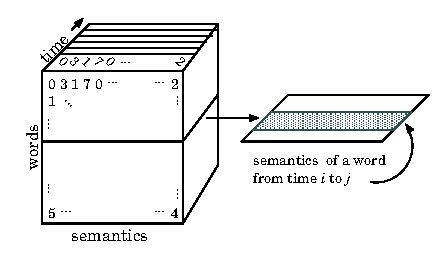
\includegraphics[width=.49\textwidth]{figures/time-tensor.eps} 
\caption{The tensor representation of the semantic space} 
\label{fig:tensor-space}
\end{figure}

\begin{figure} \center
\includegraphics[]{figures/blick-semantic-slice.eps}
\caption{The semantic slice of ``blick`` as the meaning changes due to shifts in
  word co-occurrence patterns}
\label{fig:temporal-semantics}
\end{figure}

Temporal Random Indexing can be formally described as a modification of equation
\eqref{eq:random_indexing}, with three additional equations.  As input, it takes
an annotated collection of documents $D = ( (t_0, d_0), (t_1, d_1), (t_2, d_2),
..., (t_k, d_k))$, where $d_i$ is the set of documents occurring at time $t_i$.  Let
$W_D$ be the set of all unique words in the collection.  Just as in Random
Indexing, for each word $w \in W_D$, we assign a unique index $index(w)$.  

Equation\eqref{eq:random_indexing} can then be extended to be:
\begin{equation}\label{eq:tri_temporal_semantic}
  semantics(w, t) = \sum_{c_t \in d_i} \sum_{ -n \leq i \leq n} index(w_i)
\end{equation}

where $t$ is a unique timestamp, and $c_t$ is the context for an occurrence of
$w$ at time $t$.  Using this new definition of semantics, a word slice can be
defined as:
\begin{equation}\label{eq:tri_temporal_slice}
  slice(w) = \{ (t_i, semantics(w, t_i) | w \in d_i, i=1,k \}
\end{equation}

The semantics of a word for some range of time can then easily be computed with:
\begin{equation}\label{eq:tri_temporal_snapshot}
snapshot(w, t_i, t_j) = \sum_{(t_m, s_m) \in slice(w), t_i \leq t_m \leq t_j} s_m
\end{equation}


\section{Experiments}

We applied TRI to the task of detecting events for a manually selected set of
199 words from a variety of topics.  We selected words based on how frequently
it was used in a corpus and knowledge that it would be likely to be discussed in
blogs.  However, limiting the word selection was done for efficiency, and this
approach could be applied to tracking events for a larger set of words.  Due to
limited space, we illustrate the performance using a set of six word of
divergent topics that includes both abstract and specific concepts: college,
Lebanon, nuclear, Wii, PS3, and XP.

\subsection{The Corpus}
\label{sec:corpus}

Our approach can be applied to any corpus that has a known date of authorship
of each article, at the granularity desired for analysis of semantic shifts.
For the purpose of detecting changes in public opinion over the course of recent
events, and the detection of previously unknown, but still interesting, events,
we have utilized a portion of an already existing corpus\cite{sia08efficient}.

The corpus comes from a collection of blog postings from 2004 on.  These blog
postings come from around the world, and in a variety of languages.  We view
this as an excellent example of an unstructured corpus for event detection since
it is composed of blog articles harvested by
BlogLines\footnote{http://www.bloglines.com}.  The documents come from some
standard news sources, but also from any blogging service which provides rss
feeds, such as livejournal, local newspapers, wordpress, and many more.

For this experiment, we collected only English articles from the blog corpus,
but the algorithm could be used in practice with any language.  The date of
authorship for each document in this collection is estimated to be the most
recent date the document has been updated.

Overall we expect this corpus to be well fitted to the challenge of detecting
events while handling multiple view points beyond editorial control.  Table
\ref{tab:sample_blogs} provides three sample blog posts which exemplify the
issue.  Each of the posts were written near the release of the Wii game console,
each with a significantly different usage of words, and sentiment.  There is a
clear range of styles, from the mechanical description of the device, to
opinions on the company releasing the system, and finally to adoration of the
system. Beyond this sample set of posts, the corpus meets our expectations in
other ways.  First, the lack of editorial oversight in the documents leads to
grammatical and spelling errors, and frequently to the introduction of new terms
or phrases unique to the author along with other issues\footnote{This may lead
to an increase in polysemy and synonomy amongst words, potentially impacting our
approach, but exploration of this topic is left for future work}.   Second, the
corpus has a large number of discussed topics, ranging from international
events, to product releases, and to personal musings.

\begin{table*}[tb]
\centering {\footnotesize
\begin{tabular*}{\textwidth}{ p{.3\textwidth} p{.25\textwidth}  p{.38\textwidth} }
\hline

For those of you who went, I hope you guys had just as much fun as I did. One
of the best parts was actually being able to play the Wii. When I picked up
that controller, I was sold instantly. The other awesome part was being able to
demo for Enchanted Arms in the Ubisoft area. I have a bunch of pictures up on
my  Flickr Account if people are interested.  &

With  motion-sensing controls  and three-dimensional movements on screen, the
upcoming  Nintendo Wii  game platform is changing the way video game developers
think about games.
&

While I agree that expanding video games beyond its core audience is certainly
an intriguing idea (if not necessary), it doesn't exactly thrill me as a member
of said audience.  Nintendo has already done a fine job of  turning us all into
their little marketing minions with the DS.  None of this will change with the
Wii.  I call it exploitation of the weak spot in our hearts for the big N. \\

\hline
\end{tabular*}}
\caption{Contrasting blog entries about the Wii gaming console prior to its
  release in November 2006}
\label{tab:sample_blogs}
\end{table*}

Before the corpus is used for performing event detection, the corpus is
preprocessed to render it more uniform.  Similar to other semantic space
approaches that used web-gathered data\cite{rohde09improved}, this
pre-processing allows the model to gracefully handle several irregularities in
writing style, such as inconsistent use of punctuation and capitalization.
Additionally, this process removes many tokens such as html mark-up, which have
little or no semantic content in themselves\footnote{We note that the HTML might
be interpreted to yield more information however, TRI is agnostic to its input,
and so no special HTML processing is done}.  The corpus is processed as follows:
{\small
\begin{enumerate}
  \setlength{\itemsep}{1pt}
  \setlength{\parskip}{0pt}
  \setlength{\parsep}{0pt}

  \item Replace all numbers with $<$num$>$

  \item Remove all html mark-up and email addresses

  \item Remove unusual punctuation, and separate all other punctuation from words
  
  \item Remove words of 20 characters in length
    
  \item Converting all words to lower case
  
  \item Replacing \$5 to $<$num$>$ dollars
  
  \item Discard articles with fewer than some threshold percentage of correctly
    spelled English words

  % \item Discard duplicate articles according to a 128 bit hash.
  
  \item Associate each entry with a numeric timestamp
   
\end{enumerate}}
When computing the semantics, we also impose two filters on corpus during
processing: any word in a list of frequent closed-classed words and those words
not in the most frequent 250,000 words in the blog corpus were removed.  This
step is both practical and empirically motivated.  

Removing closed-class is a common practice in semantic spaces
models\cite{rohde09improved, sahlgren08permutations}, due to the low semantic
value; words such as ``the'' or ``of'' so frequently appear that they do not
serve to distinguish the meaning of any co-occurring word.  Similarly,
infrequent words can safely be removed for initial uses due to the small effect
they would have on other semantic vectors.

For both stop words and infrequent words, their original position is preserved
after removal.  This ensures that the window for counting co-occurrence takes
into account the words originally within the window distance.  All remaining
words and tokens are assigned an index vector for computing the semantics.

We limited the analysis to the 2006 postings in the corpus; this constituted
15,725,511 blog entries and a total of 2.62 billion tokens (both words and
punctuation) after the normalization process.  

\subsection{Detecting Events using TRI}

Events are extracted using a three step process.  First, TRI is used to convert
the corpus into semantic slices.  A month-long time span was selected after an
empirical analysis of the particular corpus showed that the the reduced
frequency of words in smaller time spans led to semantics that performed less
well.  TRI was configured using 10,000 dimensional vectors with a $\pm 3$ word
window.  Index vectors had the values of 4 dimensions randomly assigned to $+1$
or $-1$, and the rest to be $0$.  Processing the entire corpus using TRI took
approximately 100 minutes on a 2.4GHz Intel Core 2 processor with 8 gigabytes of
RAM.

In the second step, the semantic shift is calculated for each word.  To detect
the shift, a word's semantic vectors for slices at time $t_i$ and $t_{i+1}$ are
compared using the cosine similarity, which measures the similarity in angle
between vectors.  The cosine similarity ranges between $1$ and $-1$, indicating
identical and opposing angles, respectively.  The semantic shift is defined as
the $1 -\ $ the cosine similarity.
Changes in angle reflect a change in a word's meaning, which in this system can
signify the presence of an event.  Changes in magnitude were also tracked but an
analysis showed they were not correlated with events.  Table
\ref{tab:shift-table} shows semantic shifts for several test words.

\begin{table*}[htb!f]
  
\begin{tabular*}{\textwidth}{  @{\extracolsep{\fill}} | r | c c c c  c c c c  c c c | }

\hline
& Feb & Mar & Apr & May & Jun & Jul & Aug & Sep & Oct & Nov & Dec \\ \hline

college & 0.00 & 0.00 & 0.00 & 0.00 & 0.05 & 0.05 & 0.00 & 0.00 & 0.00 & 0.00 & 0.00 \\ \hline 

Lebanon & 0.04 & 0.05 & 0.05 & 0.06 & {\bf 0.16} & {\bf 0.25} & 0.01 & 0.01 & 0.02 & 0.03 & 0.01 \\ \hline 

nuclear & 0.02 & 0.02 & 0.02 & 0.02 & 0.02 & 0.02 & 0.02 & 0.01 & {\bf 0.11} & 0.06 & 0.02 \\ \hline 

PS3 & 0.06 & 0.04 & 0.06 & 0.05 & 0.03 & 0.04 & 0.03 & 0.02 & 0.02 & 0.03 & 0.01 \\ \hline

Wii & {\bf 0.12} & {\bf 0.14} & {\bf 0.15} & 0.06 & 0.03 &  0.04 & 0.04 & 0.02 & 0.01 & 0.01 & 0.01 \\ \hline

XP & 0.03 & 0.04 & 0.03 & 0.03 & {\bf 0.19} & {\bf 0.20} & 0.02 & 0.02 & 0.02 & 0.02 & 0.01 \\\hline 

\end{tabular*}
\caption{Semantic shift values for six example words where bold indicates a
  significant change}
\label{tab:shift-table}
\end{table*}

The third step selects those topic words that undergo a significant semantic
shift and associate the topic words with documents.  We define the significance
for a shift in terms of its deviation from the mean semantic shift using a
simple time series analysis.  Specifically, we calculate the mean and standard
deviation for the semantic shift of all words in the two slices.  If a word's
shift is greater than one standard deviation away from the mean, then it the
word is marked as undergoing a significant shift.  The bold values in table
\ref{tab:shift-table} note these shifts for five example words.

To form the association between documents and topic words, each word that
undergoes a significant shift has its nearest neighbors calculated.  These
neighbors are often words associated with the topic word, but are not
necessarily synonyms.  We posit that the neighbors provide context about the
nature of an event by virtue of reflecting the frequent co-occurrences in the
documents.  To retrieve the event-related documents, the topic word and its
neighbors are used as query terms to search the corpus during the month that the
event occurred.  Documents are retrieved using a simple technique that returns
the posts containing the event term and the highest frequency of the related
terms.

Accurately evaluating event detection requires a set of events that are known a
priori to bein the corpus.  For large corpora with millions of documents, such
as the Bloglines corpus used here, it is infeasible to determine the complete
set of events that are present.  Furthermore, determining what kinds of events
may be present can prove problematic, as blogs frequently discuss many topics
outside the range of normal news events.  To create a baseline for evaluation,
We constructed a limited set of significant news events that were likely to be
in the corpus and then manually verified their presence.  Descriptive keywords
for each event were then to evaluate TRI.  Ultimately, the evaluation is an
analysis of not only TRI, but also the corpus itself, as some terms, or events,
may not be present at all within the corpus.  We plan to use this initial
methodology to identify a better means of analyzing massive corpora and
the diverse set of events contained therein.


\subsection{Results}

Several semantic shifts correlated well with known events of 2006.  We discuss
the results by analyzing the events detected for the words in table
\ref{tab:shift-table}.  Table \ref{tab:event-blogs} lists some of the highest
rated blogs associated with specific events our technique detected.

Both the ``Wii'' and the ``PS3'' are gaming consoles released in North America
in November 2006.  However, only the Wii experienced a significant semantic shift.
The stabilization of the semantics correlates with the products demonstration at
the Electronics Entertainment Expo, a major gaming event.  The corpus contained
many examples of attendees describing their experiences with both consoles at
the convention.  Notably the PS3 underwent only a slight shift, indicating 
a fairly stable meaning.  Further analysis showed that the change in ``Wii'' was
due to the console being renamed from ``Revolution'' to ``Wii'' in late April.

The 2006 Lebanon War took place in July 2006, which was detected by a
significant shift in meaning and is further supported by a change in the 
nearest neighbors.  In July, the nearest neighbors of ``Lebanon'' were terms
associated with war, such as ``Hezbollah'', ``soldiers'', and
``rockets''.  However, before, and after the war, the ten closest neighbors to
``Lebanon'' in 2006 were names of countries, revealing that during the course of
the war, the semantics of ``Lebanon'' shifted dramaticly to a different class of
words, and then returned to it's original class once the war concluded.

The changes for ``nuclear'' correspond directly to claims that North Korea
conducted nuclear tests in October 2006.  Until October, the related terms of
``nuclear'' are focused on Iran, and nuclear power; during
October, the neighbors shift towards terms such as ``Korea'', ``atomic'',
``sanctions'', and ``bomb.''  

Throughout the year, ``college'' experienced no noticeable semantic shifts,
despite the annual events of beginning and graduating college.  We view this as
example of a consistent word which acts as a reference point to other words.

An analysis for ``XP'' showed a semantic shift caused by an unlikely change in
corpus content; during the month of June, spammers added such a high number of
advertisements for Windows XP copies, shifting the semantics to unimportant
terms.  An examination of the nearest neighbors to ``XP'' showed a dramatic
change from related operating system terms such as ``Windows,'' ``Linux'' and
``Vista'' to numbers and currency abbreviations.

Overall, using the cosine similarity metric, and then further examining the sets
of nearest neighbors proved to be an effective method of catching semantic
shifts.  Furthermore combining the nearest neighbors with a simple document
retrieval algorithm generated relevant documents corresponding to the events
which caused the shift.

\begin{table*}[tb]
\centering {\footnotesize
\begin{tabular*}{\textwidth}{  p{.31\textwidth} p{.31\textwidth} p{.31\textwidth} }
\hline

\multicolumn{1}{c}{Lebanon} & \multicolumn{1}{c}{nuclear} & \multicolumn{1}{c}{Wii} \\
\hline

Exercising great restraint, they instantly launched airstrikes on Lebanon,
damaging critical roads, [...], power stations, etc.  Hezbollah
retaliated with a stream of rockets that penetrated as far Ashaifa, causing a
great deal of terror to Israeli civilians.

&

Pyongyang would not hold negotiations to resolve the outstanding issues with
Washington, [...] ``the Americans never recognized our security and we were
forced to conduct nuclear test to defend ourselves.''

& 

The Wii was the name of the console.. It was time to see if it could deliver its
promise of ``changing the way we game.'' Their presentation was probably the
most ``fun,'' cutting right to the chase and demonstrating uses of the
controller in games.

\\

[T]heir goal is to move public opinion in Lebanon against Hezbollah due to the
destruction ``they'' caused the country, establish a strong deterrence for any
future attacks, and , of course, destroy as much of Hezbollah's infrastructure
and weapons as possible.

&

Korea nuclear test hasn't tipped military balance [...]  hours ago questions
surrounding North Korea and its nascent nuclear weapons program took center
stage Monday night

&

It turns out, according to eyewitness reports from the show floor, that
we might not have been playing Wii consoles at the Nintendo booth...should I
feel betrayed? \\ \hline
\end{tabular*}}
\caption{Blog snippets describing events associated with  ``Lebanon'' in
July, ``nuclear'' in October, and ``Wii'' in May}
\label{tab:event-blogs}
\end{table*}



\section{Related Work}
\label{sec:related-work}

Among the many systems that perform event detection, several use a related
technique that maps documents, rather than words, into a vector space.
Documents are represented by a vector of their term frequencies, with most
approaches using some form of weighting the vectors, such as term
frequency-inverse document frequency (TF-IDF) weighting.  Additionally, many
event detection systems restrict themselves to processing newswire text, instead
of blogs.

Most document based event detection algorithms extend a core usage of TF-IDF
weighting.  In the core event detection algorithm, each document is analyzed to
produce TF-IDF values for each word occurring in the document.  This set of
values can then be compared against TF-IDF values of other documents using the
same similarity measures used in semantic space models, with cosine similarity
being one of the most common.  In general, an event is detected if the current
document is significantly different from all other processed documents, based on
a threshold of similarity values between
documents\cite{brants03ned,kumaran04entityevent}.

Brants et al. introduced some significant improvements to the standard document
based model\cite{brants03ned}.  The first improvement was to compute the TF-IDF
values on a document by document basis, allowing the system to continuously
process new documents.  The second improvement was computing a set of TF-IDF
values which were dependent on the source of the document, under the assumption
that some words, such as CNN, would be more frequent based on who wrote the
document.  Beyond modifying the TF-IDF values, the similarity measure was also
extended to include some normalization techniques that take into consideration
the source of the documents, and the average similarity of documents.  Finally,
their model was extended to compare segmentations of documents, rather than
entire documents.  Overall, these modifications showed noticeable improvements
over the basic usage of TF-IDF values and similarity metrics.

Kumaran and Allan expand on Brants et al. by considering not only the term
frequencies when computing the similarity between documents, but also named
entities, such as ``President Obama,'' in the
documents\cite{kumaran04entityevent}.  Two additional vectors are created for
each document: One composed of just the named entities occurring in a document,
and another composed of all words that are not named entities.  When comparing
the similarity between two documents, the standard vector is initially used, and
then the similarity between the additional vectors are used to provide finer
distinctions, such as whether two documents refer to the same set of named
entities, and the same set of general topics, i.e. all the non named entities.

In \cite{lam01contextual}, Lam et al. extend a document-space approach by
associating each document with three vectors: a TF-IDF weighted vector; a TF-IDF
score of named entities present in the document, similar to
\cite{kumaran04entityevent}; and a concept vector, which details which abstract
concepts are contained in the document, using TF-IDF scores based on the
frequency of concepts rather than words.  The key terms in a document are each
given a weight based on which key terms the document contains.  Event detection
is done by clustering documents as they appear.  Each cluster is said to
represent a specific event; and documents that do not fit into one cluster are
said to be new events.  Chen et al. use a similar clustering for event detection
but use sentences rather than entire document\cite{chen07hot}.

Makkonen et al. augment the document representation by using an existing
ontology to extract out locations, proper names, and temporal references
from the document\cite{makkonen04simple}.  These three, combined
with the remaining terms in the document are used as the basis for comparison.

Overall, the current event detection systems that do not utilize a semantic
space have the key benefit of being able to process documents continuously,
since no reduction step is required for vector representations.  But the key
difference is the focus on comparisons between documents, and not words that
occur in documents.  These approaches must handle different challenges, such as
documents that discuss multiple events and elements of documents that are
vague but important for distinguishing events.

\section{Discussion}

The semantic space model we have presented has a number of benefits and
drawbacks compared to other semantic space and document based techniques for
automatic event detection.  The most significant outstanding question is how to
analyze all the semantic slices produced in an efficient manner that exposes
events.  While our preliminary analysis has shown that events can be detected
using TRI, our approach does not currently scale to searching across all terms,
nor to identifying events for new words that infrequently occur.  However, we
argue that the advantages provided by TRI outweigh the outstanding issues and
merits further work to address these limitations.

Event detection systems that use semantic spaces have two notable challenges due
to how time is integrated.  First, the space must be easily modifiable as new
documents are produced.  Existing approaches use a single dimensionality
reduction step after a corpus had been processed to improve information
retrieval. However this step limits the integration of new documents into the
semantic space; to integrate new documents, the space must be completely
recomputed.  The second challenge stems from comparing word meanings and
documents that occur in different times.  Approaches such as
\cite{kontostathis04use,fortuna09visualization} that arbitrarily segment the
corpora used into different semantic spaces artificially limit both the types of
comparisons available and the specific time ranges of the semantics.  TRI
addresses both of these challenges efficiently.  By being based on Random
Indexing, dimensionality reduction is done concurrently with developing semantic
vectors.  Additionally, by utilizing the same set of index vectors over all
documents analyzed, every semantic slice is contained within the same semantic
space, avoiding the need for reference only those vectors that are common to
several time periods.

Conversely, the document based methods discussed in section
\ref{sec:related-work} provided a means of avoiding a post processing stage by
incrementally determining the TF-IDF values for words in the corpus.  While
these approaches efficiently allow the inclusion of more documents over time,
each document vector encounters similar problems seen in basic co-occurrence
semantic space models, most notably the requirement that two documents have the
same exact words for them to be declared similar.  

The introduction of additional vector representations of a document, such as the
named entity vectors, or the concept vectors, attempt to address this issue, but
these additions allude to benefits provided by a semantic space model.  For
instance, if two documents describe the same events, but without using the same
set of words, and instead use highly similar words to describe the event
differently, the document based event detection methods would either report two
distinct events, or rely on some system which can determine the similarity
between two words.  Being based on word semantics, TRI avoids this problem, and
provides a way of determining how similar two terms are, or which concepts a
word refers to.  With TRI, synonymous key words describing the event are
modified in a similar manner, and words with similar meanings will have similar
effects on the semantics.  It may also be possible with TRI to detect synonymous
event names by identifying words with similar shifts and similar neighbors.
However, further investigation is needed.

While TRI provides elegant solutions to several problems in event detection,
significant questions still remain.  First, a suitable method of analyzing the
semantic shift between vectors is needed.  Our initial experiment illustrates
tracking outliers based on cosine similarity works well in practice; however,
this does not utilize all the information present and could leave some events
undetected.  Time series analysis or probability distribution analysis are two
techniques which might be well suited for similarity comparisons between
semantic slices.
However, it remains an open question of what limitations exist to the types of
events TRI can be detected, and whether the method of comparison can be targeted
to find specific kinds of events.

As a second issue, the relationship should be established between the corpus,
the duration of a semantic slice, and the types of events that are detected.
Our current system was able to detect changes at a monthly granularity, but
real-time event detection must operate on a much finer scale.  Further work is
needed to determine how brief a semantic slice can be while still adequately
representing the semantics necessary for event detection.

Regarding the granularity of semantic slices and semantic vectors, we suspect
that the optimal granularity is highly dependent on how dense documents are with
regards to time in the corpus.  One drawback of Random Indexing is the need for
a large amount of data, and if there is not enough data, semantic vectors become
poorly defined and produce weak similarity scores.  We found that the corpus
used in the experiment was sparse enough to produce a degradation in the
semantics when our semantic slices were set to a time range shorter than a
month.  Ideally the corpus should have a dense enough set of topics for very
narrow semantic slices.

\section{Conclusion}

Unstructured, unfiltered corpora such as blogs present an ideal opportunity for
automated event-detection systems to identify new events before they can be
reported through more formal sources.  We have presented an algorithm that uses
changes in word semantics to detect new events in blog posts.  Our approach
utilizes simple word co-occurrence and scales well to processing millions of
blog posts.  Additionally, initial experiments to identify events for specific
words proved successful.  Further work is needed to identify the strengths and
weakness of this approach and quantify its ability to detect events.  However,
we plan to address these issues in future work.  Last we plan to release the
implementation of TRI as a part of the S-Space Package\cite{jurgens09sspace}.

\section*{Acknowledgements}

We thank John Cho and his lab for access to the blogline corpus used in this
work.  We also thank the anonymous reviewers for their comments and suggestions.

\bibliographystyle{abbrv} \bibliography{cml_paper}

\end{document}
